\subsection*{Estado de resultados}
\addcontentsline{toc}{subsection}{Estado de resultados}

El estado de resultados está proyectado a cinco años, de tal manera que se conocen en detalle los movimientos del flujo de dinero que se realizan dentro de la empresa, teniendo en cuenta los gastos necesarios para generar las utilidades netas de cada año fiscal.

En la tabla \ref{EstadoResultados} se ilustra la utilidad bruta, que se obtiene como la diferencia entre las ventas netas y el total del costo de ventas. Asimismo, se presenta la utilidad operativa, la cual es el resultado de restar a la utilidad bruta los gastos administrativos. Finalmente, se incluyen los gastos financieros y preoperativos, que permiten calcular la utilidad antes de impuestos; posteriormente, al descontar el impuesto de renta correspondiente al año gravable 2026, se obtiene la utilidad neta.

\begin{table}[H]
	\centering
	\caption[{Estados de resultados}]{\centering Estado de resultados. \textit{Fuente:} Autores.}
	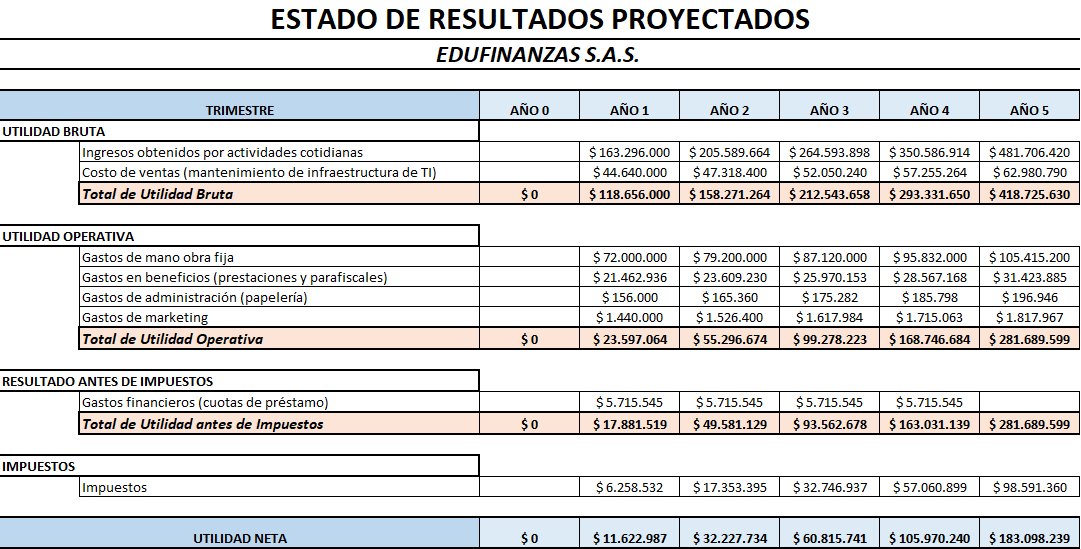
\includegraphics[width=15cm]{Imagenes/EstadoResultados.png}
	\label{EstadoResultados}
\end{table}